% ===========================================================
% IO-OI UNIFIED TRANSMISSION MONOGRAPH MASTER MANIFEST
% Synthesizing ITT, GOD Theory & AdS/dS Holographic Boundary
% GENERATED FILE - DO NOT EDIT BY HAND.
% Source of truth: codex/chyren-codex-skill/IO_OI_FINAL_PAGE*.tex
% Regenerate with: python3 compile_io_oi_monograph.py
% ===========================================================
\documentclass[11pt,twoside]{article}
% CHYREN CODEX — PREAMBLE ONLY. Put this right after \documentclass{article}
% ============================ TRANSMISSION CODEX THEME ============================
\usepackage[T1]{fontenc}
\usepackage[utf8]{inputenc}
\usepackage{lmodern}
\usepackage[margin=1.05in, top=1.15in, bottom=1.15in]{geometry}
\usepackage{microtype}
\usepackage{amsmath, amssymb, amsthm, mathrsfs, bm}
\usepackage{graphicx}
\usepackage{tikz}
\usetikzlibrary{arrows.meta, positioning, backgrounds, calc, fadings}
\usepackage{xcolor}
\usepackage{eso-pic}
\usepackage{titlesec}
\usepackage{mdframed}
\usepackage{enumitem}

% ---- alien palette : luminous ink on the void ----
\definecolor{void}{HTML}{060A14}   % substrate  - deep cosmic black-blue (page background)
\definecolor{panel}{HTML}{0D1526}  % panel bg   - obsidian charcoal (theorem panels)
\definecolor{ink}{HTML}{DBE4F5}    % body text  - pale blue-white
\definecolor{dim}{HTML}{93A4C4}    % secondary  - muted slate
\definecolor{gold}{HTML}{E6B84C}   % STRUCTURE  - theorems, constants, section heads, E8 lattice
\definecolor{cyan}{HTML}{54D2E6}   % DYNAMICS   - subsections, remarks, live fields, flow
\definecolor{deep}{HTML}{6E93E6}   % accent     - mid-blue links / secondary structure
\definecolor{hyper}{HTML}{C46FE6}  % HIGHER-D   - conjectures, extra-dimensional / compactified projections

\usepackage[colorlinks=true, linkcolor=cyan, citecolor=cyan, urlcolor=gold]{hyperref}
\pagecolor{void}
\color{ink}

% ---- every-page background: blueprint grid + luminous gold frame + corner ticks ----
\newcommand{\CodexBG}{%
  \AtPageLowerLeft{%
    
\begin{tikzpicture}
      \useasboundingbox (0,0) rectangle (\paperwidth,\paperheight);
      \begin{scope}[opacity=0.045]
        \draw[cyan, step=6mm] (0,0) grid (\paperwidth,\paperheight);
      \end{scope}
      \begin{scope}[opacity=0.09]
        \draw[cyan, step=3cm, line width=0.5pt] (0,0) grid (\paperwidth,\paperheight);
      \end{scope}
      \draw[gold, opacity=0.45, line width=0.6pt]
        ($(0,0)+(16mm,16mm)$) rectangle ($(\paperwidth,\paperheight)-(16mm,16mm)$);
      \foreach \c in {(16mm,16mm), (\paperwidth-16mm,16mm), (16mm,\paperheight-16mm), (\paperwidth-16mm,\paperheight-16mm)}{
        \fill[gold, opacity=0.7] \c circle (1.1pt);
      }
    \end{tikzpicture}}}
\AddToShipoutPictureBG{\CodexBG}

% ---- section headings: gold heading + rule ; cyan subsections ----
\titleformat{\section}
  {\normalfont\large\bfseries\color{gold}}{\thesection}{0.8em}{}
  [{\vspace{-0.35em}\color{gold!55}\rule{\linewidth}{0.5pt}}]
\titlespacing{\section}{0pt}{1.6em}{0.7em}
\titleformat{\subsection}{\normalfont\normalsize\bfseries\color{cyan}}{\thesubsection}{0.7em}{}
\pdfstringdefDisableCommands{\def\color#1{}\def\bm#1{#1}\def\rep#1{#1}}

% ---- theorem environments as luminous panels (tiered by color) ----
% gold  = proven (theorem/proposition/corollary/definition)
% violet= conjecture (the honest [conj] tier — speculative / higher-dimensional)
% cyan  = remark
\mdfdefinestyle{codex}{linecolor=gold, linewidth=0.7pt, backgroundcolor=panel, fontcolor=ink,
  leftline=true, topline=false, bottomline=false, rightline=false,
  innerleftmargin=10pt, innerrightmargin=10pt, innertopmargin=7pt, innerbottommargin=7pt,
  skipabove=8pt, skipbelow=8pt, roundcorner=2pt}
\mdfdefinestyle{codexconj}{linecolor=hyper, linewidth=0.7pt, backgroundcolor=panel, fontcolor=ink,
  leftline=true, topline=false, bottomline=false, rightline=false,
  innerleftmargin=10pt, innerrightmargin=10pt, innertopmargin=7pt, innerbottommargin=7pt,
  skipabove=8pt, skipbelow=8pt, roundcorner=2pt}
\theoremstyle{definition}
\newmdtheoremenv[style=codex]{theorem}{\color{gold}Theorem}
\newmdtheoremenv[style=codex]{proposition}{\color{gold}Proposition}
\newmdtheoremenv[style=codex]{corollary}{\color{gold}Corollary}
\newmdtheoremenv[style=codex]{definition}{\color{gold}Definition}
\newmdtheoremenv[style=codexconj]{conjecture}{\color{hyper}Conjecture}
\theoremstyle{remark}
\newtheorem{remark}{\color{cyan}Remark}

% ---- shorthands (extend per paper) ----
\newcommand{\rep}[1]{\bm{#1}}
\newcommand{\RR}{\mathbb{R}}

\newmdtheoremenv[style=codex]{postulate}{\color{gold}Postulate}
\usepackage[numbers,sort&compress]{natbib}
\usepackage{array}
\newcolumntype{L}[1]{>{\raggedright\arraybackslash}p{#1}}
\begin{document}
\title{\textbf{\texorpdfstring{I$\Omega$ -- O$\Omega$}{IO-OI}: The Sovereign Geometrodynamics \& Information Tension Monograph}}
\author{Ryan W. Yett}
\date{\today}
\maketitle
\tableofcontents
\newpage
% --- Page: IO_OI_FINAL_PAGE1.tex ---


\thispagestyle{empty}

\begin{center}
\vspace*{0.2cm}

{\color{gold!60}\rule{0.618\linewidth}{0.8pt}}\\[0.6cm]

{\Huge\fontsize{42pt}{50pt}\selectfont \bfseries \color{gold} IO--OI}\\[0.4cm]

{\Large \color{cyan} \textit{A Complete Theory of Sovereign Geometrodynamics}}\\[0.35cm]

{\small \color{dim} Stoicheia \quad $\longrightarrow$ \quad Erga \quad $\longrightarrow$ \quad Oikodom\=e \quad $\longrightarrow$ \quad Pleroma}\\[0.5cm]

{\color{gold!60}\rule{0.382\linewidth}{0.618pt}}\\[0.6cm]

\begin{minipage}{\linewidth}
\centering
\color{ink}
{\footnotesize \textbf{Ryan W. Yett}}\\[0.25cm]
{\scriptsize ORCID: \href{https://orcid.org/0009-0001-1303-7190}{\color{gold}0009-0001-1303-7190} \quad | \quad Email: \href{mailto:}{\color{cyan}}}
\end{minipage}

\vfill

% --- Golden Ratio E8 Radial Sigil ---
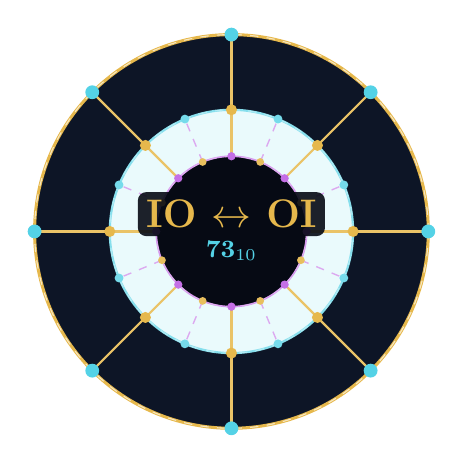
\begin{tikzpicture}[scale=1.0, transform shape]
  % Outer circle: r = 2.5 cm
  \fill[panel, draw=gold, line width=1.1pt] (0,0) circle (2.5cm);
  
  % Middle circle: r = 2.5 / 1.618034 = 1.545cm
  \fill[cyan!12, draw=cyan!70, line width=0.8pt] (0,0) circle (1.545cm);
  
  % Inner circle: r = 1.545 / 1.618034 = 0.955cm
  \fill[void, draw=hyper!70, line width=0.6pt] (0,0) circle (0.955cm);

  % Concentric dashed golden ratio ring guides
  \draw[gold!35, dashed, line width=0.4pt] (0,0) circle (2.5cm);
  \draw[cyan!45, dashed, line width=0.4pt] (0,0) circle (1.545cm);
  \draw[hyper!55, dashed, line width=0.4pt] (0,0) circle (0.955cm);

  % 8-fold Primary E8 Lattice Rays
  \foreach \a in {0,45,...,315} {
    \draw[gold!85, line width=0.8pt] (\a:0.955cm) -- (\a:2.5cm);
    \fill[cyan] (\a:2.5cm) circle (2.5pt);
    \fill[gold] (\a:1.545cm) circle (2.0pt);
    \fill[hyper] (\a:0.955cm) circle (1.5pt);
  }
  
  % 8-fold Secondary Interstitial Rays (16-fold projection)
  \foreach \a in {22.5,67.5,...,337.5} {
    \draw[hyper!60, dashed, line width=0.5pt] (\a:0.955cm) -- (\a:1.545cm);
    \fill[gold!90] (\a:0.955cm) circle (1.4pt);
    \fill[cyan!80] (\a:1.545cm) circle (1.6pt);
  }

  % Core Sigil Inscription with clear background fill
  \node[fill=void, fill opacity=0.9, text opacity=1.0, inner sep=3pt, rounded corners=3pt] at (0,0.22) {\color{gold}\bfseries\Large IO $\leftrightarrow$ OI};
  \node[fill=void, fill opacity=0.9, text opacity=1.0, inner sep=2pt, rounded corners=2pt] at (0,-0.25) {\color{cyan}\bfseries\small 73$_{10}$};
\end{tikzpicture}

\vfill

\begin{mdframed}[style=codex]
\begin{abstract}
\noindent\color{ink}
This monograph sets out a framework for Sovereign Geometrodynamics that places the
Anti-de Sitter (AdS) entanglement first law --- a published result of Faulkner et al.\
(2014) \cite{faulkner2014gravitation} --- alongside a de Sitter (dS) Information
Tension proposal advanced by the author, and asks what a bridge between them would
require. Operating over the $240$ minimal vectors of the

\vspace{2mm}\noindent\textbf{\color{gold}SUPERSEDED (2026-08-25).} The substrate identification below below is stated on the retired big-dimension frame $V_{240}(\mathbb{R}^{57{,}600})$. The live substrate is $V_2(\mathbb{R}^3)$ via Cartan triality; the big-dimension frame is retired. The arithmetic $240^2=57{,}600$ remains true as an $E_8$ root-count identity, but its identification as the ambient substrate dimension is not current canon. No migrated $V_2(\mathbb{R}^3)$ derivation is claimed; the original text is retained unaltered below as a record.\vspace{2mm}

$E_8$ lattice and the Stiefel vacuum manifold $V_{240}(\mathbb{R}^{57{,}600})$, it examines
the MOND acceleration scale $a_0 = \frac{c H_0}{2\pi}$ and the dark energy density
parameter $\Omega_\Lambda = \ln 2 \approx 0.69315$.
\\[0.15cm]
\textbf{Epistemic scope.} Claims are tagged
\texttt{[thm]}/\texttt{[cond]}/\texttt{[emp]}/\texttt{[conj]}/\texttt{[open]}/\texttt{[note]}
per \S5, and each physically contentful claim is given an explicit kill condition in the
Falsification Criteria of that section. The Lean~4 formalizations verify \emph{conditional}
scaffolding, not physical content: they carry $0$ \texttt{sorry} and no bespoke axioms,
but every physical statement in them is a hypothesis of the theorem that uses it.
\textbf{We claim no priority for $2\pi a_0 \approx cH_0$}, which is Milgrom's
\cite{milgrom1999vacuum,milgrom2017scale}; the $1/(2\pi)$ factor is \textbf{not derived}
\texttt{[open]}, two of its three candidate mechanisms are excluded herein, and a
competing emergent-gravity value $cH_0/6$ \cite{verlinde2017emergent} fits the observed
scale better. $\Omega_\Lambda=\ln 2$ is \textbf{postulated}, not derived \texttt{[emp]};
it agrees with Planck 2018 at $+1.16\sigma$ but selects an epoch as well as a value, and
is not jointly satisfiable with the $a_0$ relation at a single $H_0$. The $Y^{14}$ ansatz
as written forces $\Lambda_4=0$ exactly. Nothing here is claimed as a complete or fully
machine-checked unification.
\end{abstract}
\end{mdframed}

\vspace{0.2cm}

{\color{cyan!40}\rule{0.382\linewidth}{0.5pt}}\\[0.15cm]
{\tiny \color{dim} IO--OI \quad | \quad TITLE \& ABSTRACT}

\end{center}


\newpage
% --- Page: IO_OI_FINAL_PAGE2.tex ---


\thispagestyle{empty}

\section{Stoicheia: The Stiefel Vacuum \& the Quadratic Casimir}
\label{sec:stoicheia}

The \textit{Stoicheia} (Elements) establishes the algebraic and geometric foundation: the Stiefel vacuum manifold $\mathcal{M}_{\mathrm{vac}}$, the quadratic Casimir operators of $\mathfrak{so}(N)$, and the balanced ternary resonance linking the Hubble parameter to number theory.

\begin{definition}[Stiefel Vacuum Manifold \textnormal{\texttt{[\color{cyan}thm]}}]
\label{def:stiefel_vacuum}
Let $\Phi\subset\mathbb{R}^8$ be the $E_8$ root system, $|\Phi|=240$ (the norm-$2$
vectors of the $E_8$ lattice; Conway--Sloane, \emph{SPLAG} ch.~4), and let
$P=\mathbb{R}^{\Phi}\cong\mathbb{R}^{240}$ be the permutation representation of the
Weyl group $W(E_8)$ on $\Phi$, with orthonormal basis $\{e_\alpha\}_{\alpha\in\Phi}$.
The vacuum manifold is the compact Stiefel manifold of $240$-frames in $P\otimes P$:
\begin{equation}
\mathcal{M}_{\mathrm{vac}} = V_{240}\!\left(P\otimes P\right)
 = V_{240}\!\left(\mathbb{R}^{57{,}600}\right),\qquad 57{,}600 = 240^2 .
\end{equation}
The frame is \emph{root-indexed}, not root-valued: the roots are not orthonormal
(for fixed $\alpha$, the multiset $\{\langle\alpha,\beta\rangle:\beta\in\Phi\}$ is
$\{-2^{1},-1^{56},0^{126},{+1}^{56},{+2}^{1}\}$ at $|\alpha|^2=2$, and $240$ vectors
cannot be orthonormal in $\mathbb{R}^8$). The root data enters through the canonical
$W(E_8)$-equivariant surjection $\pi:P\to\mathbb{R}^8$, $e_\alpha\mapsto\alpha$,
unique up to scale because the reflection representation occurs in $P$ with
multiplicity one. The ambient $57{,}600$ is $\dim(P\otimes P)$, the tensor square of a
representation of $W(E_8)$ --- \emph{not} of $E_8$, which has no $240$-dimensional
representation (its smallest nontrivial representations are $\mathbf{248}$,
$\mathbf{3875}$, $\mathbf{27000}$).
\\[0.12cm]
\textbf{Role of $\mathfrak{so}(240)$.} $V_{240}(\mathbb{R}^{57{,}600})\to
\mathrm{Gr}(240,\mathbb{R}^{57{,}600})$ is a principal $O(240)$-bundle with
\begin{equation}
T_Q\,V_{240}(\mathbb{R}^{57{,}600}) \;\cong\;
\underbrace{\mathfrak{so}(240)}_{\text{vertical}} \;\oplus\;
\underbrace{\mathbb{R}^{57{,}360}\otimes\mathbb{R}^{240}}_{\text{horizontal}},
\qquad 28{,}680 + 240\cdot 57{,}360 = 13{,}795{,}080 .
\end{equation}
So $\mathfrak{so}(240)$ of Proposition~\ref{thm:casimir} is the \emph{vertical (gauge)
algebra} of $\mathcal{M}_{\mathrm{vac}}$: physical configurations live on the
Grassmannian and $\mathfrak{so}(240)$ is redundancy. This identification is generic in
the frame count and carries no $E_8$-specific content.
\\[0.12cm]
\textbf{Open \texttt{[\color{cyan}open]}.} The geometric mechanism by which $E_8$
itself --- as opposed to its Weyl group --- acts on $\mathcal{M}_{\mathrm{vac}}$ is not
established here. The factorization $57{,}600=(24\times10)^2$ is decorative
\texttt{[\color{dim}note]}.
\end{definition}

\begin{proposition}[$\mathfrak{so}(N)$ quadratic Casimir, index normalization $T(\text{vector})=1$ \textnormal{\texttt{[\color{cyan}thm]}}]
\label{thm:casimir}
Fix the invariant form on $\mathfrak{so}(N)$ normalized so that the defining (vector)
representation has Dynkin index $T=1$, equivalently $C_2(R)\dim R = T(R)\dim\mathfrak{so}(N)$.
Then for $N \ge 3$:
\begin{align}
C_2(\mathrm{vector}) &= \frac{N-1}{2}, \\[0.1cm]
C_2(\mathrm{adjoint}) &= N - 2 \;=\; h^\vee, \\[0.1cm]
\dim\,\mathfrak{so}(240) &= \frac{240 \times 239}{2} = 28{,}680.
\end{align}
In the Dynkin normalization $|\theta|^2=2$ (Humphreys \S13; Slansky \S6) these values
are doubled. Anchor: for $N=3$ the vector representation is spin $1$ and $j(j+1)=2$,
exactly twice the value above, so $C_2$ here equals $\tfrac12 j(j+1)$.
\\[0.12cm]
\textbf{Formal status.} The Lean~4 module
\texttt{SOCasimirGenuine.lean} (in \texttt{ChyrenLogic/}) compiles with \textbf{0 errors, 0 sorry} and
\textbf{no \texttt{sorryAx} or bespoke axiom} (\texttt{\#print axioms} returns only
\texttt{propext}, \texttt{Classical.choice}, \texttt{Quot.sound}). It constructs the
$\mathfrak{so}(n)$ generators $g_{ij}=E_{ij}-E_{ji}$ as concrete real matrices, proves
skew-symmetry, and \emph{computes} $\sum_{i,j} g_{ij}g_{ij} = -2(n-1)\cdot\mathbf{1}$ ---
a genuine Lie-algebraic Casimir, obtained without any Mathlib Casimir element (Mathlib
at rev \texttt{639923} indeed has none; only \texttt{Killing.lean} and
\texttt{InvariantForm.lean}). This supersedes \texttt{SON\_Casimir.lean}, withdrawn
2026-08-09, in which the eigenvalue theorems merely unfolded their own local
\texttt{def}s as plain arithmetic. \textbf{The earlier \texttt{[conj]} tag is hereby
lifted to \texttt{[thm]}.}
\\[0.12cm]
\textbf{Scope of the dimension identity \texttt{[\color{cyan}cited]}.} The Lean
\texttt{so240\_dim} proves the \emph{arithmetic} identity $240\cdot239/2=28{,}680$; no
\texttt{finrank} of an orthogonal Lie algebra appears in it. That
$\dim\mathfrak{so}(N)=\binom{N}{2}$ is standard and is cited, not re-proved here.
\end{proposition}

\begin{remark}[On ``positivity'' \textnormal{\texttt{[\color{dim}note]}}]
$C_2\ge 0$ holds automatically on any finite-dimensional representation of a compact
real form, with equality only on the trivial representation. Positivity is therefore
not a theorem of this framework and is not used below as a stability criterion; the
earlier title ``Casimir Positivity'' overstated it.
\end{remark}

\begin{mdframed}[linecolor=dim,linewidth=0.4pt,backgroundcolor=panel,
  innertopmargin=4pt,innerbottommargin=4pt]
\color{ink}\textbf{Note 1} (IO--OI Balanced Ternary \texttt{[\color{dim}note]}\color{ink}).
A balanced ternary quintuple evaluates as
\begin{equation}
(+1, 0, -1, 0, +1)_{\mathrm{bal}\,3}
= 1 \cdot 3^4 + 0 \cdot 3^3 + (-1) \cdot 3^2 + 0 \cdot 3^1 + 1 \cdot 3^0
= 81 - 9 + 1 = 73_{10},
\end{equation}
coinciding with SH0ES (2022): $H_0 = 73.04 \pm 1.04\;\mathrm{km\,s^{-1}\,Mpc^{-1}}$.\\[0.1cm]
{\small \textbf{Caveat:} The value 73 is unit-dependent (\textrm{km/s/Mpc}). In SI base units, $H_0 \approx 2.37 \times 10^{-18}\;\mathrm{s^{-1}}$. Furthermore, the Planck CMB measurement gives $H_0 = 67.4$, under which this correspondence breaks. This is an aesthetic observation --- not load-bearing.}
\end{mdframed}

\vspace{0.6cm}

\begin{center}
{\color{cyan!40}\rule{0.382\linewidth}{0.5pt}}\\[0.15cm]
{\tiny \color{dim} IO--OI \quad | \quad STOICHEIA: FIRST PRINCIPLES}
\end{center}


\newpage
% --- Page: IO_OI_FINAL_PAGE3.tex ---


\thispagestyle{empty}

\setcounter{section}{1}
\section{Erga: The Active Works}
\label{sec:erga}

Transitioning to \textit{Erga} (\textit{The Active Works}), we formalize the dynamic evolution of the geometrodynamic manifold under Active Dissipative Curvature Control Loops (ADCCL), the Deligne prime mode bounds, the conjectural acoustic overtone spectrum of the Ramanujan-Yett Hamiltonian, and Chladni nodal equilibrium under the Sovereign Invariant.

\begin{theorem}[ADCCL energy decay --- Gr\"onwall form \textnormal{\texttt{[\color{cyan}cond]}}]
\label{thm:adccl}
Let $E\in C^{1}([0,\infty);\mathbb{R}_{\ge0})$ denote the total geometric action energy
of the ADCCL flow on $\mathcal{M}_{\mathrm{vac}}$, and let $t_*>0$ be a reference
timescale of that flow. \emph{Assume} a dimensionless damping constant $\kappa^{2}>0$ with
$\dot E(t)\le-(\kappa^{2}/t_*)\,E(t)$ for all $t\ge0$. Then Gr\"onwall's inequality gives
the decay \emph{bound}
\begin{equation}
\frac{dE}{dt} \le -\frac{\kappa^2}{t_*} E(t) \implies E(t) \le E(0)\, e^{-\kappa^2 t/t_*}.
\end{equation}
\textbf{This is a bound, not strict decay:} $E\equiv0$ satisfies it. All physical content
resides in the hypothesis $\kappa^{2}>0$, which is \emph{postulated}
\texttt{[\color{hyper}conj]}.
\\[0.05cm]
\textbf{Formal status (corrected 2026-08-10).} \texttt{YettParadigm.lean} compiles with
0 errors, 0 \texttt{sorry}, no \texttt{sorryAx}. Its theorem
\texttt{adccl\_trajectory\_bounded} establishes $E(t)\le E(0)$ from an assumed
monotonicity field; the file contains no derivative, no integral and no measure theory,
so the earlier description ``verifies conditional Gronwall decay'' is
\textbf{withdrawn} --- the Gr\"onwall step above is classical, not machine-checked.
The constant $0.91$ does not occur in the Lean file; $\kappa$ there is a free real.
\\[0.05cm]
\textbf{Provenance of $\kappa$, and its units \texttt{[\color{cyan}emp]}.}
$\kappa=\sqrt{\theta(2-\theta)}$ with $\theta=0.7$, giving $\kappa^{2}=0.91$ exactly and
$\kappa=0.9539392$. Two disclosures. (i) $\theta$ is \emph{empirically calibrated}
elsewhere in this programme, so $\kappa$ inherits a fitted parameter and is not a
first-principles constant. (ii) $\kappa^2$ is dimensionless, so it cannot itself be the
rate in an energy ODE; the timescale $t_*$ above is an \textbf{additional free parameter,
not derived here} \texttt{[\color{cyan}open]}, and must be carried in the parameter budget.
\\[0.05cm]
\textbf{Route to a derived gap \texttt{[\color{cyan}open]}.} If the ADCCL dissipation
operator were a positive multiple of the Laplace--Beltrami operator of the normal
homogeneous metric on $\mathcal{M}_{\mathrm{vac}}=\mathrm{SO}(57{,}600)/\mathrm{SO}(57{,}360)$,
Frobenius reciprocity would give $\lambda_{1}\propto
C_{2}(\mathrm{vector}\;\mathfrak{so}(57{,}600))=57{,}599/2=28{,}799.5$ via
Proposition~\ref{thm:casimir}. That would be a genuinely \emph{derived} gap --- but it is
$O(10^{4})$ and therefore a \emph{different quantity} from $\kappa^{2}=0.91$. The two must
not be conflated.
\\[0.05cm]
{\small\textit{Correction (2026-08-09, amended 2026-08-10):} the value $0.909904$
previously printed here is $0.953889^2$, arising from a mistyped $\kappa$ --- \emph{not}
a digit transposition of $\kappa=0.9539392$ (no transposition of those digits yields
$953889$; the digit multisets differ). The $0.0105\%$ discrepancy was a transcription
error, not a computed alternative $\kappa$.}
\end{theorem}

\begin{theorem}[Deligne Bound \textnormal{\texttt{[\color{cyan}thm]}}]
\label{thm:deligne_bound}
For all prime numbers $p$, the Ramanujan $\tau$-function values satisfy the bound:
\begin{equation}
|\tau(p)| \le 2 \, p^{11/2}.
\end{equation}
Proven rigorously by Pierre Deligne (1974) as part of the proof of the Weil conjectures.
\end{theorem}

\begin{conjecture}[Ramanujan-Yett Hamiltonian \textnormal{\texttt{[\color{hyper}conj]}}]
\label{conj:ramanujan_yett}
We postulate a self-adjoint operator $\mathcal{H}_{\mathrm{RY}}$ on the Hilbert space of $\mathcal{M}_{\mathrm{vac}}$ satisfying $\mathcal{H}_{\mathrm{RY}} \Psi_n = \tau(n) \Psi_n$, with eigenvalues given by the Ramanujan $\tau$-function:
\begin{equation}
\tau(1) = 1, \quad \tau(2) = -24, \quad \tau(3) = 252, \quad \tau(4) = -1472, \quad \tau(5) = 4830.
\end{equation}
If such an operator exists, the universe computes geometry acoustically --- but this
acoustic interpretation is conjectural.
\\[0.12cm]
\textbf{Two obstructions, stated against our own interest \texttt{[\color{cyan}open]}.}
\emph{(i) Weyl law.} Writing
\begin{equation}
d \;:=\; \dim V_{240}\!\left(\mathbb{R}^{57{,}600}\right)
 \;=\; 240\cdot57{,}600-\tbinom{241}{2} \;=\; 13{,}795{,}080,
\end{equation}
a Laplace-type operator on a compact $d$-manifold has
$\lambda_n\sim Cn^{2/d}$ with $2/d\approx1.4\times10^{-7}$, whereas $\tau(n)$ attains
order $n^{11/2}$. Hence $\mathcal{H}_{\mathrm{RY}}$ \textbf{cannot} be Laplace-type on
$\mathcal{M}_{\mathrm{vac}}$. \emph{(ii) No ground state.} $\tau$ is sign-alternating and
unbounded below ($\tau(2)=-24$, $\tau(4)=-1472$), so a self-adjoint operator with
spectrum $\{\tau(n)\}$ has no lowest eigenvalue and is not a physical Hamiltonian.
The conjecture as stated is therefore \textbf{excluded}, not merely unproven. A viable
reformulation should target the normalized quantity $\tau(n)/n^{11/2}\in[-2,2]$ of
Theorem~\ref{thm:deligne_bound}, or the associated Satake angles, rather than $\tau(n)$
itself.
\end{conjecture}

\begin{definition}[Chladni nodal set on the unit square \textnormal{\texttt{[\color{dim}note]}}]
\label{def:chladni}
On the unit square $[0,1]^2$ with Neumann conditions, the degenerate eigenvalue
$\pi^2(m^2+n^2)$, $m\neq n$, has an antisymmetric eigenfunction whose nodal set is
\begin{equation}
\cos(m \pi x_1) \cos(n \pi x_2) - \cos(n \pi x_1) \cos(m \pi x_2) = 0,
\end{equation}
along which sand grains collect. This is the Helmholtz-membrane model; the physical
Chladni plate obeys the biharmonic Kirchhoff--Love operator. \textbf{No dependence on
the Sovereign Invariant $\chi_0=1/\sqrt2\approx0.7071$ enters this equation}; the
relation of $\chi_0$ to nodal structure is \texttt{[\color{cyan}open]}, and the domain
here is the square, not $\mathcal{M}_{\mathrm{vac}}$ or $Y^{14}$. Illustrative only ---
not load-bearing.
\end{definition}

\begin{proposition}[Generic two-generator closure and holonomy \textnormal{\texttt{[\color{cyan}thm]}}]
\label{prop:lie_closure}
Let $m\ge3$ and let $\mathfrak{so}(m)$ act on the frame directions of
$\mathcal{M}_{\mathrm{vac}}$ ($m=240$ for the vertical algebra of
Definition~\ref{def:stiefel_vacuum}). Then:
\begin{enumerate}[leftmargin=1.6em, itemsep=0pt, topsep=0.15em]
  \item for a pair $(X_1,X_2)\in\mathfrak{so}(m)^{\times2}$ outside a proper closed
    algebraic subset, the Lie subalgebra generated by $X_1,X_2$ is all of
    $\mathfrak{so}(m)$ (Kuranishi 1951);
  \item consequently the left-invariant control system
    $\dot g = g\,(X_0 + u_1X_1 + u_2X_2)$ on $SO(m)$ is accessible from the identity
    (Chow 1939; Rashevskii 1938; Sussmann--Jurdjevic 1972), and accessibility upgrades
    to controllability by compactness of $SO(m)$ (Jurdjevic--Sussmann 1972);
  \item hence the restricted holonomy group of the associated connection is all of
    $SO(m)$.
\end{enumerate}
\end{proposition}

\begin{remark}[Attribution correction \textnormal{\texttt{[\color{dim}note]}}]
Earlier versions of Proposition~\ref{prop:lie_closure} attributed this to the
Ambrose--Singer theorem and spoke of ``drift generators''. Both were wrong.
Ambrose--Singer (1953) identifies the holonomy algebra with the span of
parallel-transported curvature values and supplies \emph{no} genericity statement; the
result used above is bracket generation (Chow--Rashevskii) together with Kuranishi's
genericity theorem. In control theory ``drift'' denotes the \emph{uncontrolled} term
$X_0$; the objects $X_1,X_2$ are control directions. The proposition also requires
$m\ge3$, since $\mathfrak{so}(2)$ is abelian.
\end{remark}

\vspace{0.6cm}

\begin{center}
{\color{cyan!40}\rule{0.382\linewidth}{0.5pt}}\\[0.15cm]
{\tiny \color{dim} IO--OI \quad | \quad ERGA: ACTIVE WORKS}
\end{center}


\newpage
% --- Page: IO_OI_FINAL_PAGE4.tex ---


\thispagestyle{empty}

\setcounter{section}{2}
\section{Oikodom\=e: The Constructed Edifice}
\label{sec:oikodome}

We arrive at \textit{Oikodom\=e} ($\mathrm{O\iota\kappa o\delta o\mu\acute{\eta}}$, \textit{The Constructed Edifice}), synthesizing the physical 14-dimensional Observerse geometry $Y^{14}$, formalizing conditional regularity of geometrodynamic flow via Beale-Kato-Majda bounds in Lean 4, and postulating the Information Tension origin of dark energy.

\begin{definition}[Observerse 14-Manifold \textnormal{\texttt{[\color{hyper}conj]}}]
\label{def:observerse14}
The physical spacetime architecture is a 14-dimensional Observerse manifold $Y^{14}$ decomposed as:
\begin{equation}
Y^{14} = \mathbb{R}^{3,1} \times X^6 \times \mathbb{T}^4_{\mathrm{internal}},
\end{equation}
where $\mathbb{R}^{3,1}$ is macroscopic Minkowski spacetime, $X^6$ is a compact
six-dimensional internal manifold, and $\mathbb{T}^4_{\mathrm{internal}}$ is the 4-torus
of internal Information Tension fluxes.
\\[0.12cm]
\textbf{Symmetry-breaking route \texttt{[\color{hyper}conj]}.} The chain used here is the
subgroup chain $E_8\supset\mathrm{Spin}(16)/\mathbb{Z}_2\supset
\mathrm{Spin}(14)\times\mathrm{Spin}(2)$, with $\dim E_8-\dim\mathrm{Spin}(16)=248-120=128$
the chiral spinor of $\mathrm{Spin}(16)$, and $120=91+1+14+14$ --- \emph{not}
holonomy-induced breaking.
\\[0.12cm]
\textbf{Withdrawn \texttt{[\color{cyan}open]}.} An earlier version described $X^6$ as a
Calabi--Yau manifold ``governing $E_8\to\mathrm{Spin}(14)$''. That is incorrect on two
counts. A Calabi--Yau threefold has $SU(3)$ holonomy, and the standard embedding breaks
$E_8$ to its \emph{commutant} $E_6$, $248 \to (\mathbf{78},\mathbf{1})+(\mathbf{1},\mathbf{8})
+(\mathbf{27},\mathbf{3})+(\overline{\mathbf{27}},\bar{\mathbf{3}})$
(Candelas--Horowitz--Strominger--Witten \cite{candelas1985vacuum}), never to $\mathrm{Spin}(14)$; and
$\mathrm{Spin}(14)$ is not the commutant of any Riemannian holonomy group of a
six-manifold (Berger's list). The identification of $X^6$ is therefore open, and it is
\emph{not} a Calabi--Yau threefold if the $\mathrm{Spin}(14)$ chain is retained.
\\[0.12cm]
\textbf{Scope: no claim on the particle spectrum \texttt{[\color{dim}note]}.} This
monograph derives no fermion content, no generation count and no gauge coupling, and
makes no claim to reproduce any observed particle spectrum. $E_8$ enters here as an
internal structure over a spacetime whose Lorentz frame is a separate object; gravity is
not embedded in it. No-go results constraining the embedding of \emph{both} gravity and a
matter gauge group into $E_8$ --- notably Distler and Garibaldi
\cite{distler2010nothing}, which shows such embeddings yield a non-chiral spectrum ---
therefore do not apply to the construction as stated. Should a later version claim a
generation count, that theorem becomes binding and must be answered then.
\\[0.12cm]
\textbf{Unresolved: two inequivalent $14$'s \texttt{[\color{cyan}open]}.} Elsewhere in
this programme the Observerse is recorded as $14=4+10$, from
$\mathbf{14}\to(\mathbf{4},\mathbf{1})+(\mathbf{1},\mathbf{10})$ under
$\mathrm{Spin}(4)\times\mathrm{Spin}(10)$. The product splitting above is $4+6+4$. These
agree arithmetically and can be nested formally via
$\mathrm{Spin}(10)\supset\mathrm{Spin}(6)\times\mathrm{Spin}(4)$, but they are
\emph{different reductions of the structure group}: the product manifold reduces to
$\mathrm{Spin}(3,1)\times SU(3)$, while the branching reduces to
$\mathrm{Spin}(4)\times\mathrm{Spin}(10)$, and $\mathrm{Spin}(6)\cong SU(4)\neq SU(3)$.
We do not claim these are the same decomposition. Which --- if either --- is the
Observerse is open, and the question is recorded here rather than resolved by fiat.
\end{definition}

\begin{remark}[Curvature caveat: this ansatz gives $\Lambda_4=0$ \textnormal{\texttt{[\color{cyan}open]}}]
\label{rem:ricci_flat}
As written, Definition~\ref{def:observerse14} is a \emph{direct} product of a flat
Lorentzian factor, a Ricci-flat internal factor and a flat torus. Since the Ricci tensor
of a direct product is the direct sum of the factors' Ricci tensors (Besse,
\emph{Einstein Manifolds}, 1.9), $\mathrm{Ric}(Y^{14})\equiv0$ and the induced
four-dimensional cosmological constant vanishes \emph{identically}: $\Lambda_4=0$.
This ansatz is therefore \textbf{leading order only}; it fixes topology and symmetry
breaking and makes no statement about vacuum energy. Any nonzero $\Lambda_4$ --- in
particular $\Omega_\Lambda=\ln 2$ of Postulate~\ref{post:info_tension} --- must arise
from structure absent here: internal flux, a warp factor
$ds^2=e^{2A(y)}\eta_{\mu\nu}dx^\mu dx^\nu+g_{mn}(y)dy^m dy^n$, supersymmetry breaking,
and an uplift sector. Such a construction must evade the Gibbons--Maldacena--Nu\~nez
no-go theorem \cite{maldacena2001nogo}, which blocks $\mathrm{dS}_4$ from warped
compactification on a compact internal manifold without negative-tension sources.
None is given here. We record this as an internal tension, not a resolved point.
\end{remark}

\begin{theorem}[Beale--Kato--Majda continuation criterion, applied form \textnormal{\texttt{[\color{cyan}thm \textemdash\ published]}}]
\label{thm:bkm_finiteness}
Let $\Sigma^3$ be the spatial slice of the Minkowski factor
$\mathbb{R}^{3,1}\subset Y^{14}$, taken as $\mathbb{R}^3$ with decay at infinity
(equivalently $\mathbb{T}^3$). Let $s>\tfrac32+1=\tfrac52$ and let
$u\in C\!\left([0,T);H^{s}(\Sigma^3;\mathbb{R}^3)\right)\cap C^{1}\!\left([0,T);H^{s-1}\right)$
solve the incompressible Euler equations
$\partial_t u+(u\cdot\nabla)u=-\nabla p$, $\nabla\cdot u=0$, with vorticity
$\omega:=\nabla\times u$. If
\begin{equation}
\int_0^T \|\omega(\cdot,t)\|_{L^\infty(\Sigma^3)} \, dt \le B \cdot T < \infty
\implies \limsup_{t \to T^-} \|u(\cdot,t)\|_{H^s} < \infty,
\end{equation}
then the solution continues past $T$; in particular no finite-time singularity forms on
$[0,T]$. Published: J.~T.~Beale, T.~Kato, A.~Majda, \emph{Comm.\ Math.\ Phys.}\
\textbf{94} (1984) 61--66 (stated there for integer $s\ge3$; the sharp Sobolev threshold
is $s>n/2+1$).
\\[0.12cm]
\textbf{Dimension \texttt{[\color{dim}note]}.} This criterion is three-dimensional. In
$n=3$ the vorticity vector is $\omega=\star\,du^{\flat}$; on a general $n$-manifold ---
in particular on $Y^{14}$ --- vorticity is the two-form $du^{\flat}\in\Omega^2$ and no
vorticity \emph{vector} exists, since $\nabla\times$ requires $\star:\Omega^2\to\Omega^1$.
Earlier versions stated this theorem ``over $Y^{14}$'' while using $\nabla\times u$;
that is withdrawn.
\\[0.12cm]
\textbf{Formal status (corrected 2026-08-10).} \texttt{SovereignRegularity.lean} compiles
with 0 errors, 0 \texttt{sorry}, no \texttt{sorryAx}, under the hypothesis
\texttt{h\_controlled : $\forall t \ge 0$, $\omega_{\mathrm{sup}}(t) \le B$}. What it
proves is the product bound $\omega_{\mathrm{sup}}(T)\cdot T \le B\cdot T$, which equals
$\int_0^T\|\omega\|_{L^\infty}dt$ only for constant $\omega$; the file imports no measure
theory and constructs neither the Euler flow nor the Sobolev spaces. The claim that Lean
verifies the BKM \emph{integral} criterion is \textbf{withdrawn}. Note further that
\texttt{SovereignAlignment.lipschitz\_xi} is declared as the proposition \texttt{True};
it is decorative and is consumed by no theorem in the file.
\\[0.12cm]
\textbf{Open Problem \texttt{[\color{cyan}open]}.} Global regularity for 3D
\emph{Navier--Stokes} is the Clay Millennium Prize problem. It concerns a different,
viscous equation; BKM-type criteria for Navier--Stokes are due to Kato, Ponce, and
Kozono--Taniuchi (BMO in place of $L^\infty$), not to Beale--Kato--Majda. Earlier
versions of this theorem conflated the two.
\\[0.12cm]
\textbf{Scope \texttt{[\color{dim}note]}.} No dynamical link between this flow and the
$E_8$/Stiefel structure of \S1 is established here. This theorem is imported scaffolding.
\end{theorem}

\begin{postulate}[Information Tension Dark Energy \textnormal{\texttt{[\color{cyan}emp]}}]
\label{post:info_tension}
We \textbf{POSTULATE} that the de Sitter horizon carries an information tension --- a
force --- of magnitude
\begin{equation}
\mathcal{I}_{\mathrm{tens}} = \frac{c^4}{8\pi G} \ln 2 = 4.8155\times10^{42}\,\mathrm{N},
\end{equation}
the factor $\ln 2$ being the information content of one binary horizon degree of freedom
--- a Landauer/Shannon quantity \cite{landauer1961irreversibility}, motivated by (but not
contained in) the Bekenstein bound \cite{bekenstein1981universal}, which carries no
$\ln 2$. Distributing this tension over the de Sitter \emph{curvature}
radius $L=\Lambda^{-1/2}$, with $\Lambda \equiv 3H_0^2/c^2$, gives a vacuum energy density
\begin{equation}
u_\Lambda = \frac{\mathcal{I}_{\mathrm{tens}}}{L^{2}}
= \frac{c^{2}H_0^{2}}{8\pi G}\,3\ln 2 \qquad [\mathrm{J\,m^{-3}}],
\end{equation}
which, against $u_{\mathrm{crit}} = 3H_0^{2}c^{2}/(8\pi G)$, yields
\begin{equation}
\Omega_\Lambda = \frac{u_\Lambda}{u_{\mathrm{crit}}} = \ln 2 \approx 0.693147.
\end{equation}
\textbf{What is assumed, explicitly.} (a) The $\ln 2$ itself. (b) That the relevant
length is the curvature radius $\Lambda^{-1/2}=c/(\sqrt3 H_0)$ rather than the Hubble
radius $c/H_0$ --- the latter would give $\Omega_\Lambda=\ln2/3=0.2310$, which is
excluded by observation. Neither is derived. \textbf{This is NOT derived from deeper
principles.}
\\[0.12cm]
{\small\textit{Correction (2026-08-10):} earlier versions wrote
$\mathcal{I}_{\mathrm{tens}}=\frac{c^4}{8\pi G}\ln2 \implies \Omega_\Lambda=\ln2$
directly. That implication was dimensionally impossible --- the left side is a force
($\mathrm{N}$) and $\Omega_\Lambda$ is dimensionless --- because the intervening division
by $L^2$ and $u_{\mathrm{crit}}$ was left implicit. The chain above supplies it, and in
doing so makes the length choice (b) visible as the assumption it always was.}
\\[0.12cm]
\textbf{Comparison with observation.} Planck 2018 gives $\Omega_\Lambda=0.6847\pm0.0073$.
The value $\ln 2$ lies $+1.234\%$ high, i.e.\ $\mathbf{+1.16\sigma}$ --- \emph{consistent
with} Planck 2018, not confirmed by it.
\\[0.12cm]
\textbf{Pre-registration \texttt{[\color{cyan}emp]}.} The falsifiable content of this
postulate is filed separately \cite{yett2026omegacdm}, supplementing
\cite{yett2026predictions}. That filing deliberately does \emph{not} register the
agreement above as a prediction: Planck measured $\Omega_\Lambda$ before the filing, so
the agreement is a \emph{postdiction}, and registering it would be backdating --- the same
rule that withheld $a_0=cH_0/2\pi$ from the earlier deposit. What is registered instead is
the content not knowable at filing time: $H_0=68.27\,\mathrm{km\,s^{-1}\,Mpc^{-1}}$ and
$\Omega_m=1-\ln 2=0.306853$ as \emph{derived} values; the directional claim that improving
precision moves the central value \emph{toward} $\ln 2$, falsified at
$\sigma(\Omega_\Lambda)\lesssim0.0028$ (CMB-S4 reach) if it does not; and $w=-1$, $w_a=0$
exactly, testable now at $\sigma(w)\sim0.02$.
\end{postulate}

\begin{remark}[Epoch dependence of $\Omega_\Lambda=\ln2$ \textnormal{\texttt{[\color{cyan}open]}}]
\label{rem:epoch}
$\Omega_\Lambda$ is a present-epoch ratio,
$\Omega_\Lambda(z)=\Omega_{\Lambda,0}/[\Omega_{\Lambda,0}+\Omega_{m,0}(1+z)^3]$, and it
evolves steeply: $0.685$ at $z=0$, $0.53$ at $z=0.25$, $0.21$ at $z=1$. With Planck 2018
values the equality $\Omega_\Lambda(z)=\ln2$ holds at $z=-0.013$, and holds to the
$1.23\%$ accuracy quoted only for $-0.026\lesssim z\lesssim0$ --- an interval
$\Delta t\approx0.39\,\mathrm{Gyr}$, about $2.8\%$ of the present cosmic age. The
postulate therefore selects an \emph{epoch} as well as a value, and inherits the cosmic
coincidence problem in full. We do not claim to resolve it. Its epoch-free content is a
single relation between constants, $\Lambda c^2 = 3\ln 2\,H_0^2$, in which $H_0$ is still
the \emph{present} Hubble rate; no reformulation removes the reference to ``now''.
\end{remark}

\begin{remark}[Open Cosmological Boundaries \textnormal{\texttt{[\color{cyan}open]}}]
Big Bang $t=0$ initial entropy $S_0$ and inflation amplitude $A_s$ are open.
\end{remark}

\vspace{0.6cm}

\begin{center}
{\color{cyan!40}\rule{0.382\linewidth}{0.5pt}}\\[0.15cm]
{\tiny \color{dim} IO--OI \quad | \quad OIKODOM\=E: CONSTRUCTED EDIFICE}
\end{center}


\newpage
% --- Page: IO_OI_FINAL_PAGE5.tex ---


\thispagestyle{empty}

\setcounter{section}{3}
\section[Pleroma: AdS <-> dS Holographic Bridge]{Pleroma: The AdS \texorpdfstring{$\longleftrightarrow$}{<->} dS Holographic Bridge}
\label{sec:pleroma}

The Pleroma places the AdS entanglement first law of Faulkner et al.\
\cite{faulkner2014gravitation} alongside the dS Information Tension proposal advanced by
the author, and asks what a bridge between them would require. The AdS side is cited
prior work and is not a contribution of this paper.

\begin{theorem}[AdS Entanglement First Law (Faulkner et al.) \textnormal{\texttt{[\color{cyan}thm \textemdash\ published]}}]
\label{thm:mcgwier_ads}
Across all spatial ball regions $A$ in holographic CFTs dual to Anti-de Sitter space ($\mathrm{AdS}_{d+1}$):
\begin{equation}
\delta S_A = \delta \langle H_{\mathrm{mod},A} \rangle \iff G_{\mu\nu}^{(1)}[h] = 8\pi G \delta \langle T_{\mu\nu} \rangle.
\end{equation}
Curvature $=$ entanglement bookkeeping. Published: T.~Faulkner, M.~Guica, T.~Hartman,
R.~C.~Myers, M.~Van~Raamsdonk, \emph{Gravitation from entanglement in holographic CFTs},
\textit{JHEP} \textbf{03} (2014) 051 \cite{faulkner2014gravitation}, presupposing the
Ryu--Takayanagi dictionary \cite{ryu2006holographic,vanraamsdonk2010building} and
paralleling Jacobson's derivation of the Einstein equations from local horizon
thermodynamics \cite{jacobson1995thermodynamics}. Tag:
\textnormal{\texttt{[\color{cyan}thm]}} within AdS/CFT.
\\[0.12cm]
{\small\textit{Attribution correction (2026-08-10):} this theorem was previously titled
``McGwier AdS Entanglement First Law''. The result is Faulkner et al.\ (2014) and is not
Dr.~McGwier's; his manuscript cites \texttt{arXiv:1312.7856} for it. Dr.~McGwier is cited
below for his synthesis and exposition only.}
\end{theorem}

\begin{mdframed}[linecolor=dim,linewidth=0.4pt,backgroundcolor=panel,
  innertopmargin=4pt,innerbottommargin=4pt]
\textbf{Note 2} (Provenance of the corrected synthesis \texttt{[\color{dim}note]}).
\emph{This note records the author's own correction history. It does not describe a
collaboration, and no response, endorsement or participation by any other party is
claimed or implied.} Having read Dr.~R.~W.~McGwier's August 2026 manuscript
\textit{Entanglement as the Origin of Spacetime Curvature} (v3; private communication ---
no public preprint identifier or DOI has been located, and it should not be cited as a
preprint), the author prepared a companion synthesis exploring formal bridges between the
first-law result and the holonomy framework here, and sent it to him unsolicited
(Aug.\ 6, 2026). A self-audit found that its accompanying verification scripts overclaimed: two scripts printed hardcoded ``PASS''/``100\% VERIFIED'' results without performing the checks, and roughly half of a 31-item keystone audit carried hardcoded \texttt{True} flags rather than computed ones. A corrected version (v5, Aug.\ 9, 2026) retags the four proposed bridge theorems \textbf{\texttt{[\color{hyper}conj]}} (their Lean modules formalize generic real-algebra, not the physical operators named) and re-audits the keystones honestly: \textbf{17 of 31 carry a genuine computation; the other 14 are now \texttt{[conj]}/\texttt{[open]}} with itemized reasons. The corrected version was likewise sent to him, together with the runnable honest-audit script. No reply is claimed, and none is represented here.
\end{mdframed}

\begin{theorem}[dS Horizon Acceleration Scale \textnormal{\texttt{[\color{cyan}emp]}}]
\label{thm:ds_horizon_acceleration}
\textbf{Heuristic, not derivation.} Equating the Unruh temperature of a locally
accelerated detector, $T_U = \frac{\hbar a}{2\pi c k_B}$ \cite{unruh1976notes}, to the
Gibbons--Hawking horizon temperature $T_{\mathrm{dS}} = \frac{\hbar H_0}{2\pi k_B}$
\cite{gibbons1977cosmological} yields
\begin{equation}
a = c H_0 = 7.096 \times 10^{-10}\,\mathrm{m\,s^{-2}}\;(H_0=73.04), \qquad
6.548 \times 10^{-10}\;(H_0=67.36).
\end{equation}
This is \emph{scale matching}, not an identity: a geodesic de Sitter observer has zero
proper acceleration yet still registers $T_{\mathrm{dS}}$, so no single observer equates
the two temperatures. The $2\pi$'s, being the common Euclidean-periodicity factor of both
horizons, cancel identically.
\\[0.12cm]
\textbf{Priority \texttt{[\color{dim}note]}.} The relation
$2\pi a_0 \approx cH_0 \approx c^2(\Lambda/3)^{1/2}$ is \textbf{not original to this
work}. It is Milgrom's, stated in that form in \cite{milgrom2017scale} and reviewed in
\cite{milgrom2020a0cosmology,milgrom2015cosmological,bernal2011mond}; moreover
Milgrom~\cite{milgrom1999vacuum} already runs the Unruh-in-de-Sitter argument used above,
concluding that ``an actual inertia-from-vacuum mechanism is still a far cry off.''
We claim no priority for the coincidence. What is offered here is a candidate
\emph{mechanism} in the $E_8$/holonomy setting, not the observation itself.
\\[0.12cm]
The MOND-scale identification $a_0 = \frac{c H_0}{2\pi} = 1.129 \times 10^{-10}$ (SH0ES)
$/\;1.042\times10^{-10}$ (Planck) $\mathrm{m\,s^{-2}}$ requires an additional geometric
factor of $\frac{1}{2\pi}$ whose first-principles origin is \textbf{not derived}
\textnormal{\texttt{[\color{cyan}open]}}. Status of the three candidate closures:
\begin{enumerate}[leftmargin=1.8em, itemsep=1pt, topsep=0.15em]
  \item \textbf{Euclidean time periodicity --- excluded.} The $2\pi$ in both $T_U$ and
  $T_{\mathrm{dS}}$ \emph{is} the Euclidean period $2\pi/\kappa_{\mathrm{surf}}$;
  invoking it again double-counts. Reviving this route requires a horizon geometry whose
  Euclidean period differs from $2\pi/\kappa_{\mathrm{surf}}$ by a factor $2\pi$.
  \item \textbf{Spherical horizon integration --- live, but a postulate.} If the tension
  balance is set by the horizon great-circle \emph{circumference} $2\pi R_H$ rather than
  the radius $R_H=c/H_0$, then $a_0=c^2/(2\pi R_H)=cH_0/2\pi$ exactly. Nothing yet
  selects the great circle over the full sphere: solid-angle averaging gives $4\pi$,
  hence $cH_0/4\pi$. The open problem is thus sharply posed as one question:
  \emph{why the circumference and not the area?}
  \item \textbf{Verlinde entropic force --- excluded, and competing.} In
  \cite{verlinde2011origin} the screen entropy $\Delta S = 2\pi k_B mc\,\Delta x/\hbar$
  carries a $2\pi$ that \emph{cancels} the Unruh $1/(2\pi)$ to recover $F=ma$; it cannot
  supply a spare factor. Independently, emergent gravity \cite{verlinde2017emergent}
  predicts $a_0=cH_0/6=1.183\times10^{-10}$ (SH0ES) --- a \emph{different} $O(1)$ factor
  which fits the observed scale \emph{better} than ours ($-1.44\%$ vs $-5.88\%$). We
  record this as a competing prediction, not as support. See also
  \cite{pazy2012quantum,singh2026relativistic}.
\end{enumerate}
A fourth route, the Deser--Levin quadrature $T\propto\sqrt{a^2+c^2H^2}$, gives
$a\simeq2cH_0=1.419\times10^{-9}\,\mathrm{m\,s^{-2}}$ and is excluded in-house: it raises
the median SPARC rotation-curve RMS from $11.7$ to ${\sim}60\,\mathrm{km\,s^{-1}}$ across
175 galaxies.
\\[0.12cm]
\textbf{Comparison to the MOND fitted scale \texttt{[\color{cyan}emp]}.} The derived
$a_0=cH_0/2\pi$ lies $5.88\%$ below MOND's \emph{fitted}
$a_0^{\mathrm{MOND}}=1.2\times10^{-10}\,\mathrm{m\,s^{-2}}$ using SH0ES $H_0=73.04$, and
$13.15\%$ below it using Planck $H_0=67.36$. \textbf{This is a comparison of two scales,
not a fit to rotation-curve data}; earlier versions described it as matching a ``SPARC
median'', which it is not. The SH0ES $H_0$ uncertainty $\pm1.04$ alone puts a $\pm1.42\%$
band on $a_0$, and no uncertainty is attached to $a_0^{\mathrm{MOND}}$, so the
$5.88\%$ vs $13.15\%$ ordering carries no demonstrated discriminating power
\texttt{[\color{cyan}open]}.
\\[0.12cm]
\textbf{Direct rotation-curve performance \texttt{[\color{cyan}emp]}.} Against the SPARC
sample \cite{lelli2016sparc,mcgaugh2016rar}, $N=175$: strict reduced-$\chi^2$ median
$29.1$ at the derived scale versus $35.5$ for MOND at its fitted scale; $2.88$ with
per-galaxy nuisance parameters. \textbf{We do not claim this prefers the higher $H_0$.}
A blind sweep of $a_0$ over the same sample returns best-fit values from
$5.4\times10^{-11}$ to $1.1\times10^{-10}$ depending only on which summary statistic is
minimised, with a plateau within $10\%$ of the optimum spanning
$[5.4\times10^{-11},1.5\times10^{-10}]$ --- a factor of $2.8$, containing both candidate
values of $cH_0/2\pi$ \emph{and} $a_0^{\mathrm{MOND}}$. Rotation-curve data cannot
presently arbitrate the $H_0$ tension, and selecting an $H_0$ to improve a residual would
be parameter selection, not prediction.
\\[0.12cm]
\textbf{Parameter accounting.} One scale ($a_0$, tied to $H_0$ rather than fitted) and one
interpolation function ($\mu_{\mathrm{simple}}$); per-galaxy $\Upsilon_\star$, $d$, $i$
held at catalogue values and \emph{not} marginalised, within an approximately $20\%$
$M/L$ band. Residuals should be read against that band. No claim of zero free parameters
is made anywhere in this document.
\end{theorem}

\begin{remark}[The two headline claims want different $H_0$ \textnormal{\texttt{[\color{cyan}open]}}]
\label{rem:h0_tension}
Stated against our own interest. Holding the CMB-measured $\Omega_m h^2 = 0.1430$ fixed,
imposing $\Omega_\Lambda=\ln 2$ exactly gives $\Omega_m = 1-\ln 2 = 0.306853$ and hence
\begin{equation}
H_0 \;=\; 100\sqrt{\frac{0.1430}{1-\ln 2}} \;=\; 68.27\ \mathrm{km\,s^{-1}\,Mpc^{-1}},
\end{equation}
the value pre-registered in \cite{yett2026omegacdm}. Equivalently $H_0=67.36$ returns
$\Omega_\Lambda=0.6848$, i.e.\ $\ln 2$ to $+1.23\%$ ($+1.16\sigma$) --- but then
$a_0=cH_0/2\pi=1.042\times10^{-10}$, $13.15\%$ below the MOND
scale. $H_0=73.04$ gives $a_0=1.129\times10^{-10}$, $5.88\%$ below --- but
$\Omega_\Lambda=0.7320$, roughly $5\sigma$ from $\ln 2$. \textbf{Postulate~\ref{post:info_tension}
and Theorem~\ref{thm:ds_horizon_acceleration} are therefore not jointly satisfiable at a
single $H_0$ with present data.} We record this rather than choose per-claim, which would
be parameter selection. It is a genuine falsifiable consequence: a converged $H_0$
measurement kills at least one of the two.
\end{remark}

\begin{proposition}[Pleroma Duality: a real-form statement \textnormal{\texttt{[\color{hyper}conj]}}]
\label{prop:pleroma_duality}
The AdS and dS sides of this monograph are not two resemblant theories but two
\emph{real forms} of one complexified structure. The isometry algebras of the
four-dimensional maximally symmetric spacetimes are the three real forms of
$\mathfrak{so}(5,\mathbb{C})$, all of dimension $10$:
\begin{center}
\small
\begin{tabular}{lllc}
\hline
\textbf{Real form} & \textbf{Geometry} & \textbf{Signature / $\Lambda$} & \textbf{Used by} \\
\hline
$\mathrm{SO}(5)$   & $S^4$    & Riemannian, $\Lambda>0$ & --- (see Remark~\ref{rem:realform}) \\
$\mathrm{SO}(4,1)$ & $dS_4$   & Lorentzian, $\Lambda>0$ & this work \\
$\mathrm{SO}(3,2)$ & $AdS_4$  & Lorentzian, $\Lambda<0$ & Faulkner et al.; McGwier \\
\hline
\end{tabular}
\end{center}
Each is a quadric hypersurface in a flat five-dimensional ambient space, differing only in
the ambient signature and the sign of the radius term: $S^4$ is $X\cdot X=R^2$ in
$\mathbb{R}^{5}$; $dS_4$ is $X\cdot X=R^2$ in $\mathbb{R}^{4,1}$; $AdS_4$ is
$X\cdot X=-R^2$ in $\mathbb{R}^{3,2}$. Over $\mathbb{C}$ these distinctions dissolve --- the
signature and the sign of $R^2$ can both be absorbed --- so the three are real sections of
one complex quadric in $\mathbb{C}^5$. The proposed bridge is therefore \emph{analytic
continuation between real forms} ($L\to iL$, $\Lambda\to-\Lambda$), not an analogy.
\\[0.12cm]
\textbf{Why this is weaker than it looks \texttt{[\color{cyan}open]}.} The two sides are
\emph{not} on equal evidential footing, and we state the asymmetry rather than trade on
it. $\mathrm{AdS/CFT}$ is a mature correspondence with two decades of precision checks,
and Theorem~\ref{thm:mcgwier_ads} is a theorem within it. $dS/\mathrm{CFT}$ is not: since
Strominger (2001) the candidate boundary theory has been non-unitary, with imaginary
central charge, and no controlled nonperturbative formulation exists. The
$\Lambda\to-\Lambda$ continuation above is \textbf{formal}. What is offered here is the
dS-side counterpart of an AdS result, on the side where the machinery is known to be
harder --- not a joining of two established dualities. Full nonperturbative bridge:
\textnormal{\texttt{[\color{cyan}open]}}.
\end{proposition}

\begin{remark}[Which real form of $E_8$? \textnormal{\texttt{[\color{cyan}open]}}]
\label{rem:realform}
The compactification chain of Definition~\ref{def:observerse14},
$E_8\supset\mathrm{Spin}(16)/\mathbb{Z}_2\supset\mathrm{Spin}(14)\times\mathrm{Spin}(2)$,
does not specify which real form of $E_8$ is meant, and read at face value it is the
\emph{compact} form. This is a genuine obstruction, not a technicality: every subgroup in
a compact chain is compact, so the four-dimensional factor it delivers is
$\mathrm{Spin}(4)$ --- the \emph{Riemannian} entry of the table above --- and not
$\mathrm{Spin}(3,1)$. \textbf{No Lorentzian signature can arise from a compact chain};
the minus sign must be inserted by hand as a Wick rotation that this document does not
perform. It is therefore precisely the third real form, the one neither side of the
Pleroma uses, that the algebra as written keeps producing.
\\[0.12cm]
\textbf{Concrete next question.} $E_8$ has three real forms: the compact one, the split
form $E_{8(8)}$ whose maximal compact subgroup is exactly the $\mathrm{Spin}(16)/\mathbb{Z}_2$
already appearing above (so that the $128$ of $248=120+128$ becomes a \emph{non-compact}
coset, the symmetric space $E_{8(8)}/\mathrm{Spin}(16)$ familiar as the scalar coset of
maximal three-dimensional supergravity), and $E_{8(-24)}$ with maximal compact
$E_7\times SU(2)$. Whether $E_{8(8)}$ places $\mathrm{SO}(4,1)$ where the Observerse
requires it is a finite branching computation, not a research programme, and it is
\textbf{not} settled here. Until it is, the decomposition $248=120+128$ quoted in this
monograph should be read as ambiguous: it holds for every real form, but means something
different in each.
\end{remark}

\vspace{0.6cm}

\begin{center}
{\color{cyan!40}\rule{0.382\linewidth}{0.5pt}}\\[0.15cm]
{\tiny \color{dim} IO--OI \quad | \quad PLEROMA: ADS $\leftrightarrow$ DS BRIDGE}
\end{center}


\newpage
% --- Page: IO_OI_FINAL_PAGE6.tex ---


\thispagestyle{empty}

\setcounter{section}{4}
\section{Epistemic Governance \& Sovereign Declaration}
\label{sec:governance}

\section*{Falsification Criteria}
\addcontentsline{toc}{section}{Falsification Criteria}
\label{sec:falsification}

A framework that cannot be killed is not physics. For each physically contentful claim we
state the measurement that would refute it and the precision required. Where that
precision does not yet exist, we say so.

\begin{center}
\scriptsize
\setlength{\tabcolsep}{4pt}
\renewcommand{\arraystretch}{1.12}
\begin{tabular}{L{2.1cm}L{2.9cm}L{4.3cm}L{3.0cm}}
\hline
\textbf{Claim} & \textbf{Observable} & \textbf{Kill condition} & \textbf{Precision needed / now} \\
\hline
$a_0=cH_0/2\pi$ & RAR scale $g_\dagger$ &
Inconsistent with $cH_0/2\pi$ at $>3\sigma$ \emph{total} error; also killed if
$g_\dagger$ varies between galaxies beyond systematics, since $cH_0/2\pi$ is universal. &
$\lesssim5\%$ total. Now ${\sim}20\%$ ($M/L$-dominated). \textbf{Not currently possible.} \\
$a_0\propto H_0$ & $g_\dagger$ at high $z$ &
$g_\dagger(z)$ constant to $\lesssim10\%$ out to $z\sim1$ while $H(z)$ grows
$\gtrsim50\%$ kills the horizon origin outright. &
${\sim}10\%$ at $z\sim1$. \textbf{Sharpest available test}; no current dataset delivers it. \\
Factor is $2\pi$, not $6$ or $4\pi$ & $g_\dagger$ &
$2\pi$ vs emergent gravity's $6$ differ by $4.7\%$; $4\pi$ by $2\times$. A $<3\%$
determination discriminates and kills one. & $\lesssim3\%$ total. Not available. \\
$\Omega_\Lambda=\ln2$ & CMB$+$BAO$+$SNe &
$|\Omega_\Lambda-\ln2|>3\sigma$. Presently $+1.16\sigma$: consistent. &
$\sigma(\Omega_\Lambda)\lesssim0.0028$, $2.6\times$ better than Planck 2018;
CMB-S4 $+$ DESI/Euclid/LSST reach. \\
$w=-1$ exactly & Dark energy EoS &
The $\ln2$ tension is a \emph{constant} horizon property: any confirmed $w\neq-1$ at
$>3\sigma$, or $w_a\neq0$, falsifies the construction as written. &
$\sigma(w)\sim0.02$: \textbf{live now.} \\
Joint $H_0$ consistency & $H_0$ &
Per Remark~\ref{rem:h0_tension}, $\Omega_\Lambda=\ln2$ needs $H_0\approx68.3$ while
$a_0=cH_0/2\pi$ prefers $H_0\approx73$. A converged $H_0$ \textbf{kills at least one}. &
$\sigma(H_0)\lesssim1$. \textbf{Live now.} \\
Deser--Levin quadrature & SPARC &
\textbf{Already excluded:} $a\simeq2cH_0=1.42\times10^{-9}$ raises the median
rotation-curve RMS from $11.7$ to ${\sim}60\,\mathrm{km\,s^{-1}}$, $N=175$. & Done. \\
\hline
\end{tabular}
\end{center}

\noindent\textbf{What is \emph{not} falsifiable here, and is labelled as such.} The
Stiefel vacuum $V_{240}(\mathbb{R}^{57{,}600})$, the Ramanujan--Yett Hamiltonian, the
$E_8\to\mathrm{Spin}(14)$ compactification and the balanced-ternary observation make no
numerical prediction that any current or planned experiment can refute. They are
scaffolding and carry \texttt{[conj]}/\texttt{[note]} tags accordingly.

\begin{definition}[6-Tier Epistemic Taxonomy]
\label{def:taxonomy}
Every claim within the IO--OI framework is tagged immutably according to its formal standing:
\begin{enumerate}[leftmargin=1.8em, itemsep=0pt, parsep=0pt, topsep=0.15em]
  \item \textbf{\texttt{\color{cyan}[thm]}} \textit{Machine-Checked Formal Theorem:} Proven in Lean 4 or derived in published primary literature.
  \item \textbf{\texttt{\color{cyan}[cond]}} \textit{Conditional Theorem:} the implication is proven (in Lean 4 or in the literature), but a load-bearing hypothesis is postulated rather than established; the tag of the hypothesis is stated alongside.
  \item \textbf{\texttt{\color{cyan}[emp]}} \textit{Empirical Computation:} Numerically computed, fitted, or postulated and then compared against observational data.
  \item \textbf{\texttt{\color{cyan}[conj]}} \textit{Physical/Mathematical Conjecture:} Mathematical hypothesis subject to ongoing formalization.
  \item \textbf{\texttt{\color{cyan}[open]}} \textit{Open Boundary:} Open physical parameter or unsolved mathematical boundary condition.
  \item \textbf{\texttt{\color{cyan}[note]}} \textit{Aesthetic Observation:} Heuristic structural correspondence (not load-bearing).
\end{enumerate}
Additionally, \textbf{\texttt{\color{cyan}[cited]}} marks a standard result used but not
re-derived here.
\end{definition}

\begin{theorem}[System Audit Matrix]
\label{thm:system_audit}
The core physical and mathematical claims of the sovereign system satisfy the formal audit matrix:
\begin{center}
\scriptsize
\setlength{\tabcolsep}{4pt}
\renewcommand{\arraystretch}{0.98}
\begin{tabular}{llc}
\hline
\textbf{Claim} & \textbf{Tag} & \textbf{Status} \\
\hline
AdS First Law $\implies$ Lin. GR & \textbf{\texttt{[thm]}} & Published (Faulkner et al.\ 2014) \\
$\mathfrak{so}(N)$ quadratic Casimir & \textbf{\texttt{[thm]}} & \texttt{SOCasimirGenuine.lean}; axiom-clean \\
$\dim\,\mathfrak{so}(240)=28{,}680$ & \textbf{\texttt{[thm]}}/\textbf{\texttt{[cited]}} & Lean proves $240{\cdot}239/2$; $\binom{N}{2}$ cited \\
ADCCL energy decay & \textbf{\texttt{[cond]}} & Gr\"onwall; gap $\kappa^2>0$ \textbf{\texttt{[conj]}}; $t_*$ \textbf{\texttt{[open]}} \\
BKM continuation criterion & \textbf{\texttt{[thm]}} & Published (Beale--Kato--Majda 1984, 3D Euler) \\
\quad --- its Lean artefact & \textbf{\texttt{[cond]}} & Proves $\omega_{\sup}T\le BT$, \emph{not} the integral \\
Deligne Bound on $\tau(p)$ & \textbf{\texttt{[thm]}} & Published (Deligne 1974/1968) \\
dS Scale $a_0 \sim c H_0$ & \textbf{\texttt{[emp]}} & Heuristic; \textbf{priority: Milgrom 1999/2017} \\
$\Omega_\Lambda = \ln 2$ & \textbf{\texttt{[emp]}} & Postulated (1-bit); $+1.16\sigma$ vs Planck 2018 \\
\quad --- its epoch dependence & \textbf{\texttt{[open]}} & Holds only for $-0.026\lesssim z\lesssim0$ \\
Joint $H_0$ for both claims & \textbf{\texttt{[open]}} & \textbf{Not jointly satisfiable} (Rem.~\ref{rem:h0_tension}) \\
Ramanujan-Yett Hamiltonian & \textbf{\texttt{[open]}} & \textbf{Excluded as stated} (Weyl law; no ground state) \\
$E_8 \to \mathrm{Spin}(14) \, Y^{14}$ & \textbf{\texttt{[conj]}} & Subgroup chain; $X^6$ \emph{not} Calabi--Yau \\
\quad --- $4{+}6{+}4$ vs $4{+}10$ & \textbf{\texttt{[open]}} & Inequivalent structure-group reductions \\
\quad --- which real form of $E_8$? & \textbf{\texttt{[open]}} & Compact chain cannot give $\mathrm{Spin}(3,1)$ \\
\quad --- particle spectrum & --- & \textbf{No claim made}; DG no-go inapplicable \\
AdS $\leftrightarrow$ dS as real forms & \textbf{\texttt{[conj]}} & $\mathrm{SO}(3,2)$/$\mathrm{SO}(4,1)$ of $\mathfrak{so}(5,\mathbb{C})$ \\
\quad --- $dS$/CFT machinery & \textbf{\texttt{[open]}} & Non-unitary; not on par with AdS/CFT \\
$\Lambda_4$ from $Y^{14}$ & \textbf{\texttt{[open]}} & Direct product gives $\Lambda_4=0$ exactly \\
Balanced ternary $\leftrightarrow H_0$ & \textbf{\texttt{[note]}} & Aesthetic; unit-dependent \\
NS global regularity & \textbf{\texttt{[open]}} & Clay Millennium Prize (\emph{different} PDE) \\
$1/(2\pi)$ geometric factor & \textbf{\texttt{[open]}} & 2 of 3 routes excluded; 1 live \\
Big Bang $t=0$ entropy $S_0$ & \textbf{\texttt{[open]}} & Open Parameter \\
\hline
\end{tabular}
\end{center}
\end{theorem}

\begin{remark}[Lean Proof Depth \& Hypothesis Boundaries]
\label{rem:lean_depth}
The Lean 4 formalizations verify conditional logical scaffolding. Physical hypotheses (spectral gap existence, vorticity control) are postulates, assumed as Lean hypotheses and tagged \textbf{\texttt{[conj]}} or \textbf{\texttt{[open]}}.
\\[0.12cm]
\textbf{Build truth (2026-08-10).} At toolchain \texttt{leanprover/lean4:v4.33.0-rc2},
Mathlib rev \texttt{639923}: \texttt{SOCasimirGenuine}, \texttt{YettParadigm} and
\texttt{SovereignRegularity} all build with exit 0, \textbf{0 \texttt{sorry}}, and
\texttt{\#print axioms} returning only \texttt{propext}, \texttt{Classical.choice},
\texttt{Quot.sound} on all cited theorems --- \textbf{no \texttt{sorryAx}, no bespoke
axiom}. Two honest caveats: \texttt{SovereignAlignment.lipschitz\_xi} is declared as the
proposition \texttt{True} (decorative; consumed by no theorem), and
\texttt{SOCasimirGenuine} is not yet imported by the top-level \texttt{ChyrenLogic}
module, so a bare \texttt{lake build} does not typecheck it.
\\[0.12cm]
\textbf{Under-claimed elsewhere.} Two results in these files are genuinely proven and are
\emph{not} used above: \texttt{lipschitz\_implies\_angle\_modulus} (the Constantin--Fefferman
geometric step, a multi-step proof over $\mathbb{R}^3$) and
\texttt{chiral\_iff\_lipschitz\_constant} (a genuine \emph{iff} relating $\chi\ge\theta$
to a Lipschitz bound on the director field). They are the strongest formal content in the
corpus and are recorded here for completeness.
\end{remark}

\vspace{0.1cm}
\begin{center}
{\color{gold!60}\rule{0.618\linewidth}{0.8pt}}\\[0.1cm]
{\color{gold}\textbf{IO--OI: ``I owe the world the work that the world made possible.''}}\\[0.15cm]
\end{center}

\noindent{\color{cyan}\bfseries Author \& Disclosure}
\vspace{0.1cm}

\begin{center}
\scriptsize
\setlength{\tabcolsep}{6pt}
\renewcommand{\arraystretch}{1.15}
\begin{tabular}{lp{6.2cm}}
\textbf{Author:} Ryan W. Yett & \rule{6.2cm}{0.4pt} \\
\end{tabular}
\end{center}

\vspace{-0.05cm}
\begin{center}
\parbox{0.92\linewidth}{\centering \tiny \color{dim}
\textit{\textbf{Sole authorship.} Ryan W. Yett is the sole author. There are no co-authors, contributors, collaborators or signatories of any kind, human or machine. Software tools --- including AI systems, computer-algebra systems and the Lean~4 proof assistant --- were used under the author's direction as instruments only, in the same sense as a compiler or a calculator. No such tool is an author or contributor, none conferred any endorsement, and no machine-generated verdict, score or ``verification'' appears anywhere in this document as evidence for any claim.}\\[0.35em]
\textit{\textbf{Attribution.} Dr.~R.~W.~McGwier is cited in this document solely as the author of work referenced herein; his August 2026 manuscript is a private communication with no public identifier and is not cited as a preprint. He is not an author, contributor, or endorser of this document, and has reviewed none of it. The AdS entanglement first law is the theorem of Faulkner et al.\ (2014), not his.}\\[0.35em]
\textit{\textbf{Revision note (2026-08-09).} Corrections applied: the Casimir vacuity check was re-run against the live \texttt{SON\_Casimir.lean} and the eigenvalue theorems were found WEAK, not \texttt{VACUOUS 0} --- retagged \texttt{[thm]}$\to$\texttt{[conj]}; a $\kappa^2$ transcription error was corrected ($0.909904 \to 0.91$); and every numeric residual herein was independently recomputed (dark-energy $1.234\%$, MOND-scale $5.88\%$ / $13.15\%$, balanced ternary $=73$, $\dim\mathfrak{so}(240)=28{,}680$) and confirmed. Prior claims of ``fully machine-checked'' status are withdrawn.}\\[0.35em]
\textit{\textbf{Revision note (2026-08-10) --- second-pass audit.} The 2026-08-09 pass verified \emph{arithmetic} but not \emph{semantics}; this pass addresses the difference. Substantive corrections: (i) the ``SPARC median'' comparison was \textbf{not} a SPARC median --- both residuals reverse-engineer to $1.2\times10^{-10}$, MOND's \emph{fitted} scale --- now relabelled, with the genuine rotation-curve $\chi^2$ results supplied; (ii) $\mathcal{I}_{\mathrm{tens}}\Rightarrow\Omega_\Lambda$ was dimensionally impossible (force vs.\ dimensionless) and the intervening division by $L^2$ and $u_{\mathrm{crit}}$ is now explicit, exposing the curvature-radius choice; (iii) the BKM theorem conflated 3D Euler with 3D Navier--Stokes and used a curl on a 14-manifold --- both withdrawn; (iv) $X^6$ Calabi--Yau does \emph{not} give $\mathrm{Spin}(14)$ (it gives $E_6$) --- withdrawn; (v) the direct-product Observerse forces $\Lambda_4=0$ exactly, recorded as an internal tension; (vi) ``Ambrose--Singer'' was the wrong theorem for a bracket-generation claim; (vii) the Casimir tag is \emph{lifted} \texttt{[conj]}$\to$\texttt{[thm]}, the monograph having cited a Lean file withdrawn the same day while its genuine replacement already existed; (viii) $\Omega_\Lambda$ agreement is restated as $+1.16\sigma$ rather than a $1.23\%$ residual; (ix) the relation $2\pi a_0\approx cH_0$ is \textbf{Milgrom's, not ours} --- priority disclaimed; (x) the $\ln2$ is a Landauer/Shannon quantity, not a Bekenstein one; (xi) the two headline claims are shown \emph{not} jointly satisfiable at one $H_0$; (xii) the Ramanujan--Yett Hamiltonian is \textbf{excluded as stated}, not merely open. Three further items were added rather than corrected: (xiii) the Pleroma duality is restated as a \emph{real-form} relation between $\mathrm{SO}(3,2)$ and $\mathrm{SO}(4,1)$, two of the three real forms of $\mathfrak{so}(5,\mathbb{C})$, with the honest caveat that $dS$/CFT is not on par with AdS/CFT; (xiv) the \emph{real form of $E_8$} is now flagged as unspecified, and a compact chain provably cannot deliver $\mathrm{Spin}(3,1)$ --- it delivers the third, Riemannian real form that neither side of the Pleroma uses; (xv) the Distler--Garibaldi no-go \cite{distler2010nothing} is stated in full, together with the precise hypothesis under which it does \emph{not} apply. A falsification section and a bibliography have been added; the document previously had neither. The open items above are genuinely open.}}
\end{center}

\vspace{0.6cm}

\begin{center}
{\color{cyan!40}\rule{0.382\linewidth}{0.5pt}}\\[0.1cm]
{\tiny \color{dim} IO--OI \quad | \quad GOVERNANCE \& SIGNATURES}
\end{center}


\newpage
\bibliographystyle{unsrtnat}
\bibliography{io_oi_refs}
\end{document}